\documentclass{article}
\usepackage{gensymb, amsmath, float, graphicx}
\restylefloat{table}
\usepackage[margin=0.75in]{geometry}
\usepackage{verbatim}
\usepackage{multicol}
\begin{document}

\title{Ocean Bowl Bootcamp 4: Wind Patterns and Alternative Energy}
\author{Michael Shen}
\date{November 9, 2014}
\maketitle

\section{Quick Summary}

\begin{itemize}
	\item Just like the water in the oceans, the air in the atmosphere is a fluid. For this reason, it flows in directions according to the \textbf{Coriolis Effect}. In fact, the global wind patterns help define and constructively interfere with \textbf{ocean gyres}. However, there are a few key differences to remember:
	
	\item In general, global wind patterns alternate every $30\degree$ latitude: the \textbf{tradewinds}, \textbf{westerlies}, and \textbf{polar easterlies} (Figure 1). Note that winds are named from where they come from, \textit{e.g.} westerlies blow from the west to the east.
	
	\item At every multiple of $30\degree$, there is little wind. At the equator, the region is called the \textbf{Intertropical Convergence Zone (ITCZ)} or the \textbf{doldrums}. At $30\degree$ N and S, the region is called the \textbf{horse latitudes}. $60\degree$ and $90\degree$ have no special names (Figure 1).
	
	\item There is little wind in the aforementioned regions because the air is instead moving vertically! The equator receives direct sunlight, therefore the warmer air that is heated at the equator rises, later sinking at the horse latitudes.
	\begin{itemize}
		\item The same phenomenon is responsible for \textbf{land and sea breezes}. Since water has a higher \textbf{specific heat} than the shore, it heats up slower. This causes the heated air above the warmer land to rise and the cooler air above the water to sink during the day time, creating a cell and generating a sea breeze (the breeze comes from the sea towards the land). The opposite process occurs after sunset to generate a land breeze (Figure 2).
	\end{itemize}
	
	\item There is lateral wind up in the atmosphere at the boundaries, most notably the \textbf{Jet Stream}, which is at the boundary between the Westerlies and Polar Easterlies. This is widely used for air travel to save fuel (think of it as a wind current) and forms a tangible boundary. During 2013's \textbf{polar vortex} conditions, the jet stream was south of us, exposing us to the weather from the northeast, \textit{i.e.} the North Pole. This phenomenon goes by the name \textbf{nor'easter} in the New England region.
	
	\item \textbf{Low air pressure} corresponds to more clouds (increasing the chance of storms), \textbf{high air pressure} corresponds to clear skies.
	
	\item Here are a couple alternative energy sources to know: \textbf{Wind Power}, \textbf{Tidal Power}, \textbf{Wave Power}, \textbf{Ocean Current Power}, \textbf{Solar Power}, \textbf{Ocean Thermal Energy Conversion (OTEC)}, \textbf{Hydroelectric Dams}.
	\begin{itemize}
		\item Of the above, OTEC is probably the one that is unfamiliar. \textbf{Open cycle} systems (Figure 3) utilize the \textbf{thermocline} (warm surface seawater and cold seawater further down), to generate energy. It has a secondary benefit of creating freshwater as a waste product, however it is barely efficient enough to run. \textbf{Closed cycle} systems also utilize the thermocline but do not use the seawater itself, using chemicals like ammonia instead, which has a much lower boiling point. This boosts efficiency of the overall system, but introduces many other costs and challenges.
		\item The rest, with the exception of solar, utilize lateral movement of wind and water to spin a turbine, generating electricity (Figure 4). If you didn't know how electricity was generated, it's basically by spinning a magnet.
		\item Solar energy is harvested by exciting electrons into trap states in semiconductors. How these actually work is not important for Ocean Bowl and actually requires some understanding of quantum mechanics.
	\end{itemize}
\end{itemize}

\section{Figures}

\begin{figure}[H]
\centering
	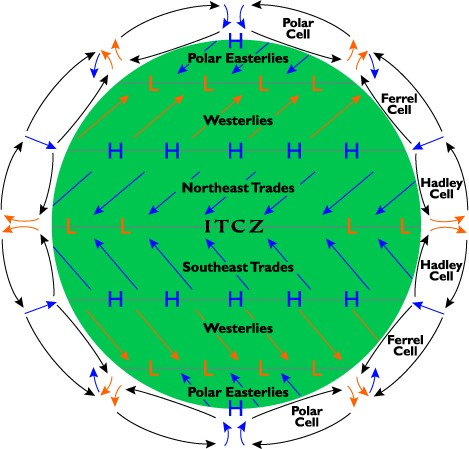
\includegraphics[scale=0.6]{./Images/BC4_WindPattern.jpg}
	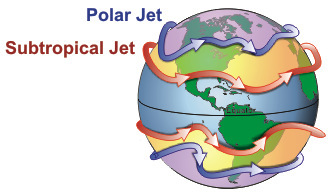
\includegraphics[scale=0.8]{./Images/BC4_JetStream.jpg}
	\caption{Simple models of the global wind patterns}
\end{figure}

\begin{multicols}{2}
\setlength{\premulticols}{1pt}
\setlength{\postmulticols}{1pt}
\setlength{\multicolsep}{1pt}
\setlength{\columnsep}{2pt}


\begin{figure}[H]
\centering
	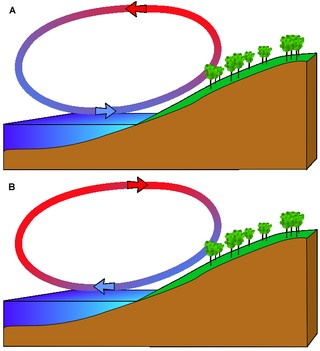
\includegraphics[scale=0.4]{./Images/BC4_LSBreeze.jpg}
	\caption{A sea and land breeze, respectively}
\end{figure}
\begin{figure}[H]
\centering
	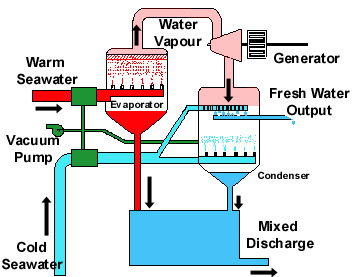
\includegraphics[scale=0.51]{./Images/BC4_OTEC.jpg}
	\caption{Open cycle OTEC system.}
\end{figure}
\end{multicols}

\begin{figure}[H]
\centering
	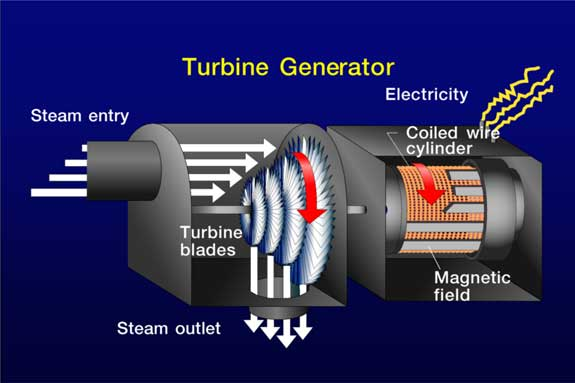
\includegraphics[scale=0.5]{./Images/BC4_Turbine.jpg}
	\caption{Electricity generation using a turbine}
\end{figure}

\end{document}